\def\sphoyear{2019}
\setcounter{section}{0}
% Headers and Descriptions
\fancyhead[L]{\textbf{SPhO \sphoyear}} \fancyhead[R]{\textbf{Questions}}


\begin{titlepage}
\centering

{\Huge\bfseries SPhO \sphoyear}

\vspace{1cm}

{\LARGE Problem Set}

\vspace{2cm}

{\Large Compiled by: Tan Chien Hao, \texttt{www.tchlabs.net}}

\vspace{2cm}

{\Large Edited/Proofread by: Keith Chan, Sun Yu Chieh, Nigel Heng}
%Collaborators please feel free to add on!

\vspace{2cm}

{\large Suggest changes at: \github}


\vfill

{\itshape Last edited: \today}
\end{titlepage}


\begin{problem}
    A projectile is fired with velocity $v_{0}$ at an angle $\theta$ to the horizontal.
    \begin{subproblem}
    The trajectory of the projectile intersects two points, both of which are at a height $h$ above the horizontal. Derive an expression for the horizontal distance $D$ between the two points.
    \hfill{[7]}\end{subproblem}
    \begin{subproblem}
    If the projectile is fired with an initial velocity of $\qty{200}{\m\per\s}$, and the barrel of the gun is angled to achieve maximum range, calculate the value of $D$.
    \hfill{[3]}\end{subproblem}
\end{problem}

\begin{problem}
    \begin{subproblem}
        A $\qty{0.25}{\kg}$ mass is attached to an unstretched spring with force constant $\qty{20}{\N\per\m}$. The mass is released and oscillates with decaying amplitude, eventually coming to rest. The process is thermodynamically irreversible. Assuming that the temperature of the surroundings remains constant at $\qty{27}{\degreeCelsius}$, calculate the change in entropy of the surroundings.
    \hfill{[4]}\end{subproblem}
    \begin{subproblem}
        The intensity of sunlight reaching the surface of the Earth is $\qty{1.37e3}{\W\per\square\m}$. Given that the radius of the Sun is $\qty{6.957e5}{\km}$, and the orbital radius of the Earth about the Sun is $\qty{1.496e8}{\km}$, estimate the surface temperature of the Sun.
    \hfill{[3]}\end{subproblem}
    \begin{subproblem}
        Given that the orbital radius of Mars about the Sun is $\qty{2.280e8}{\km}$, estimate the equilibrium temperature of Mars. 
    \hfill{[3]}\end{subproblem}
\end{problem}

\begin{problem}
    \begin{subproblem}
        A particle of mass $\qty{0.1}{\kg}$ oscillates in simple harmonic motion about a point $O$. The force acting on the particle is $F=-10 x\;\unit{\N}$, where $x\;\unit{\m}$ is the displacement of the particle about $O$. The particle begins at a distance of $\qty{0.05}{\m}$ away from $O$ with speed $\sqrt{3}/2\;\unit{\m\per\s}$. Calculate:
        \renewcommand{\theenumi}{(\alph{enumi})}
        \begin{enumerate}
            \item the amplitude
            \item the initial phase
            \item the maximum speed and acceleration of the particle\hfill{[4]}
        \end{enumerate}
    \end{subproblem}
    \begin{subproblem}
        A rod of length $L$ and uniform cross-section is partially submerged vertically in a liquid, with a length $h<L$ exposed above the liquid. Show that the rod exhibits simple harmonic motion when given a small displacement, and derive an expression for the period of the motion.
    \hfill{[6]}\end{subproblem}
\end{problem}

\begin{problem}
    \begin{subproblem}
        The electric potential at the surface of a spherical oil droplet is $\qty{1000}{\V}$. If two such droplets of equal charge and radius coalesce to form a single spherical droplet, what is the electric potential at the surface of the resulting droplet? You may assume charge is conserved.
    \hfill{[5]}\end{subproblem}
    \begin{subproblem}
        In a helium dilution refrigerator, ${}^{3}\mathrm{He}$ and ${}^{4}\mathrm{He}$ are mixed in a special chamber to obtain extremely low temperatures. The isotopes are sent through a Bainbridge mass spectrometer.
        \renewcommand{\theenumi}{(\alph{enumi})}
        \begin{enumerate}
            \item The strengths of the electric and magnetic fields in the spectrometer are $\qty{100}{\V\per\m}$ and $\qty{0.2}{\tesla}$ respectively. Calculate the speed of an ion which passes successfully through the velocity filter.\hfill{[2]}
            \item Deduce if the spectrometer can resolve the two isotopes if the exit slit of the velocity filter is $\qty{1}{\mm}$ wide.\hfill{[3]}
        \end{enumerate}
    \end{subproblem}
\end{problem}

\begin{problem}
    \begin{subproblem}
        A beam of monochromatic light of intensity $\qty{50}{\W\per\square\m}$ is incident normally onto a perfectly reflecting surface. Determine the pressure exerted on the surface.
    \hfill{[5]}\end{subproblem}
    \begin{subproblem}
        Positronium is a bound hydrogenic system with an electron orbiting a positron. The positron has the same mass as an electron, but carries a charge of $+|e|$ instead of $-|e| .$ Calculate the shortest wavelength of the Lyman series of the positronium system.
    \hfill{[5]}\end{subproblem}
\end{problem}

\begin{problem}
    A projectile is fired with velocity $\qty{50}{\m\per\s}$ from the edge of a cliff, which is at a height of $\qty{100}{\m}$ above sea level. The projectile hits a target located at a horizontal distance of $\qty{300}{\m}$ from the base of the cliff (which is at sea level).
    \begin{subproblem}
        Calculate the angle of inclination at which the projectile was fired.
    \hfill{[4]}\end{subproblem}
    \begin{subproblem}
        Suppose that instead, at the instant the projectile was fired, the target begins to move away from the cliff at a constant speed of $\qty{10}{\m\per\s}$. The angle of inclination remains the same as obtained in the previous part. Calculate the required initial speed of the projectile for it to hit the target.
    \hfill{[5]}\end{subproblem}
\end{problem}

\begin{problem}
    \begin{subproblem}
        A source $\mathrm{S}$ and a detector $\mathrm{D}$ are placed $\qty{120}{\m}$ apart. S produces sound waves of wavelength $\qty{1.33}{\m}$. A reflecting surface parallel to the line joining S and D is initially placed $\qty{90}{\m}$ away as shown below.
        
        \begin{figure}[h]
	        \centering
        	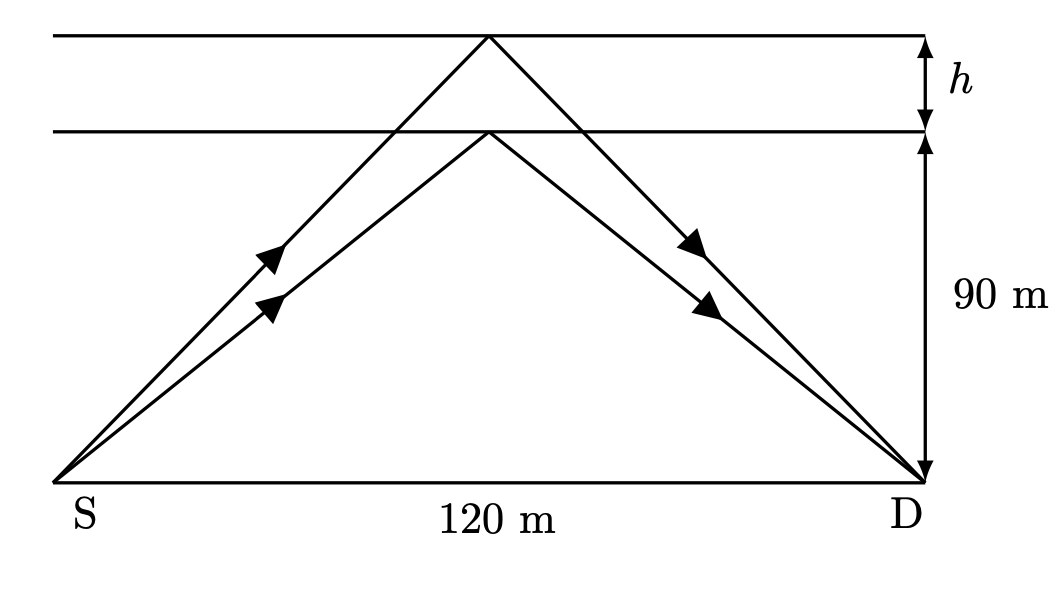
\includegraphics[width=0.5\linewidth]{spho_book_TYS_images/2019q7.png}
        	\label{2019q7}
        \end{figure}
        \noindent The sound waves directly from $\mathrm{S}$ and those reflected off the surface are found to be in phase at $\mathrm{D}$ and the intensity is at a maximum. The reflecting surface is then moved away from the line joining S and D by a distance $h$. How much should $h$ be for the intensity to be at the next maximum?
    \hfill{[5]}\end{subproblem}
    \begin{subproblem}
        A sonometer wire has diameter $\qty{0.51}{\mm}$ and is made of a material of density $\qty{8.885e3}{\kg\per\cubic\m}$. It is stretched tightly over two bridges placed $\qty{60}{\cm}$ apart. The tension in the wire is produced by hanging a uniform metal cylinder of diameter $\qty{5.0}{\cm}$ and height $\qty{10.0}{\cm}$ from the free end of the wire. The metal cylinder is slowly lowered into a liquid until half its volume is immersed. It is found that when the sonometer wire is vibrating in its second harmonic mode, the frequency of vibration is $\qty{118.4}{\Hz}$. The metal cylinder is then completely immersed in the liquid. The new frequency of vibration of the second harmonic is $\qty{114.7}{\Hz}$. Calculate the densities of the metal cylinder and the liquid.
    \hfill{[7]}\end{subproblem}
\end{problem}

\begin{problem}
    \begin{subproblem}
        A uniform hollowed sphere has inner and outer radii $r$ and $R$ respectively. Taking the gravitational potential at infinity to be zero, determine the ratio of the gravitational potential at the outer surface to that at the inner surface.
    \hfill{[5]}\end{subproblem}
    \begin{subproblem}
        A uniform cylindrical copper rod of length $\qty{30.0}{\cm}$ and diameter $\qty{2.0}{\cm}$ is well-lagged such that the heat loss through the sides is negligible. One end of the rod is in thermal contact with a large heat reservoir maintained at temperature $\qty{200}{\degreeCelsius}$, while the other is in thermal contact with another large heat reservoir maintained at $\qty{0}{\degreeCelsius}$. Calculate the rate of change of entropy of the system. [The thermal conductivity of copper is $\qty{400}{\W\per\m\per\K}$.]
    \hfill{[3]}\end{subproblem}
    \begin{subproblem}
        An electron, travelling at speed $\qty{2.08e6}{\m\per\s}$, collides with a stationary hydrogen atom with orbital angular momentum $\hbar$. Given that the energy levels of the hydrogen atom are
        \[E_{n}=-\frac{13.6}{n^{2}}\;\mathrm{eV} \text { for } n \in \mathbb{N}\]
        what are the possible wavelengths of the photons emitted by the hydrogen atom after the collision?
    \hfill{[4]}\end{subproblem}
\end{problem}

\begin{problem}
    \begin{subproblem}
        A negatively-charged particle of mass $m$ and charge $-q$ is placed at the centre of a uniformly charged ring of radius $a$ and linear charge density $\lambda$. The particle is constrained to move along the central axis of the ring, and is displaced by a distance $x\ll a$ along the axis. Given that the electric field along the central axis at a distance $x$ from the centre of a ring of radius $a$ and charge $Q$ is
        \[E=\frac{Q}{4 \pi \epsilon_{0}} \frac{x}{\left(a^{2}+x^{2}\right)^{\frac{3}{2}}}\]
        show that the particle exhibits simple harmonic motion, and determine the oscillation frequency.
    \hfill{[6]}\end{subproblem}
    \begin{subproblem}
        In the Bohr model of the hydrogen atom, when the atom is in its ground state, the electron orbits the stationary proton with radius $\qty{5.3e-11}{\m}$. The speed of the electron in the ground state orbit is $\qty{2.2e6}{\m\per\s}$. Determine the magnitude of the magnetic field at the centre of the orbit due to the electron.
    \hfill{[3]}\end{subproblem}
    \begin{subproblem}
        A circular disc of radius $R$ and surface charge density $\sigma$ spins at a rate of $n$ revolutions per second. Determine the magnetic field at the centre of the disc.
    \hfill{[3]}\end{subproblem}
\end{problem}

\begin{problem}
    \begin{subproblem}
        A particular event occurs at the origin of an inertial frame S at time $t=0$. Another event occurs at $x=\qty{4}{\cm}, y=z=0$, and $t=\qty{5}{\s}$ as measured in $\mathrm{S} .$ Determine the velocity of the inertial frame S', relative to S, in which the two events occur at the same point in space, as well as the time interval between the two events as measured by an observer in S'.
    \hfill{[6]}\end{subproblem}
    \begin{subproblem}
        A cube of side length $l$ moves at a relativistic speed $u$ with one of its sides parallel to the $x$-axis of an inertial frame S. An observer moves along the $x$-axis of S with relativistic speed $v$. Derive an expression for the volume of the cube as measured by the observer.
    \hfill{[6]}\end{subproblem}
\end{problem}